%%% CONCLUSION



\begin{frame}
\frametitle{Conclusion and perspectives}
\textcolor{midnightblue}{\large \textbf{Conclusion}}
\invisible<1>{
\begin{itemize}
\item
We proposed several numerical schemes for variational inequalities. 
\item We devised a posteriori error estimates with $\Pp$ finite elements distinguishing the error components.
\item
Adaptive stopping criteria $\Rightarrow$ reduction of the number of iterations.
\item
 Our a posteriori analysis works for unsteady problems (Two-phase flow with phase transition). 
\end{itemize}
\invisible<2>{
\textcolor{midnightblue}{\large \textbf{Perspectives}}
\begin{itemize}
\item Extension of the stationary contact problem to a hyperbolic contact problem between two vibrating membranes.
\item
Devise a posteriori error estimators for HHO
\item
Construct a posteriori error estimates for a multiphase multi compositional flow with several phase transitions.
\end{itemize}
\invisible<3>{
}}}
\end{frame}
%

%% REMERCIEMENTS + SLIDE RESERVE
\begin{frame}
\begin{overprint}

\onslide<1>
\vspace{0.3 cm}
\begin{center}
\LARGE{\textcolor{midnightblue}{Acknowledgements}}
\end{center}
\begin{itemize}
\item 
Martin Vohral\'{i}k (INRIA Paris)
\item
Vincent Martin (UTC Compiègne)
\item 
 Ibtihel Ben Gharbia (IFPEN)
 \item 
 Guillaume Delay (LJLL)
 \item 
 Soleiman Yousef (IFPEN)
 \item 
 Jean-Charles Gilbert (INRIA Paris)
\end{itemize}
\vspace*{0.2 cm}
\begin{center}
\Huge{\textcolor{black}{Thank you for your attention}}
\end{center}

%%%%%
   \onslide<2> 

\textcolor{cadmiumgreen}{\textbf{Discretization flux reconstruction:}}
\begin{equation*}
\begin{array}{lclcc}
\left({\bm \sigma}_{\ialf h, \mathrm{disc}}^{\kk,\ii,\ba}, \tauh\right)_{\omah}- \left(\gamma_{\ialf h}^{\kk,\ii,\ba},\nab {\cdot} \tauh\right)_{\omah}
&=& -\left(\mu_\ialf \psiha \nab u_{\ialf h}^{\kk,\ii,\ba}, \tauh \right)_{\omega_h^{\ba}}
&  \forall \tauh\in \Vspaceha, \\
\left(\nab {\cdot} {\bm \sigma}_{\ialf h, \mathrm{disc}}^{\kk,\ii, \ba}, q_{h}\right)_{\omah}
&=&\left(\tilde{g}_{\ialf h}^{\kk,\ii,\ba}, q_{h}\right)_{\omah}
&  \forall q_{h}\in \Qspaceha,
\end{array}
\end{equation*}
\begin{equation*}
\tildgialfhkia \egaldef \left(f_\ialf -(-1)^{\ialf} \tildlambhkia -\rialfhki \right) \psiha- \mu_\ialf \nab \uialfhki {\cdot} \nab \psiha : \mbox{\textcolor{cadmiumgreen}{depends on the residual}} 
%\left(f_\ialf -(-1)^{\ialf} \tildlambhkia -\rialfhki \right) \psiha- \mu_\ialf \nab \uialfhki {\cdot} \nab \psiha
\end{equation*}
\begin{minipage}[c]{0.4 \linewidth}
For each internal vertex $ \ba \in \Vhint$
\vspace{-0.2 cm}
\begin{equation*}
\begin{split}
\Vspaceha & \egaldef
 \left\{\tauh  \in \RTp(\omah), \, \tauh {\cdot} \nnomah=0  \mbox{ on } \partial \omah \right\}\\
\Qspaceha &  \egaldef \Pp^{0}(\omah)
\end{split}
\vspace{-0.2 cm}
\end{equation*}

\invisible<1>{
\begin{equation*}
{\bm \sigma}_{\ialf h, \mathrm{disc}}^{\kk,\ii} \egaldef \sum_{\ba \in \mathcal{V}_h} {\bm \sigma}_{\ialf h, \mathrm{disc}}^{\kk,\ii,\ba}
\end{equation*}
}
\end{minipage}
\hfill
\begin{minipage}[c]{0.5 \linewidth}
\begin{figure}
  %\begin{overprint}
    %\onslide<1>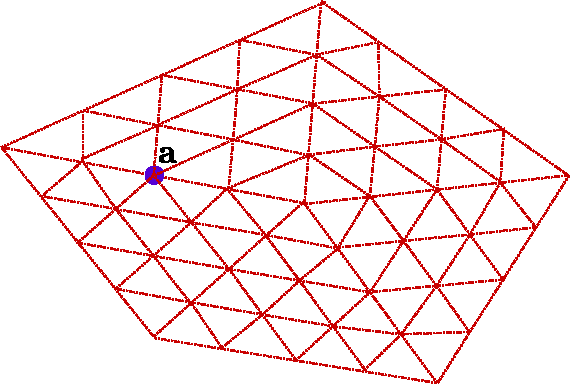
\includegraphics[width=0.84\textwidth]{patch_alg_3.pdf}
    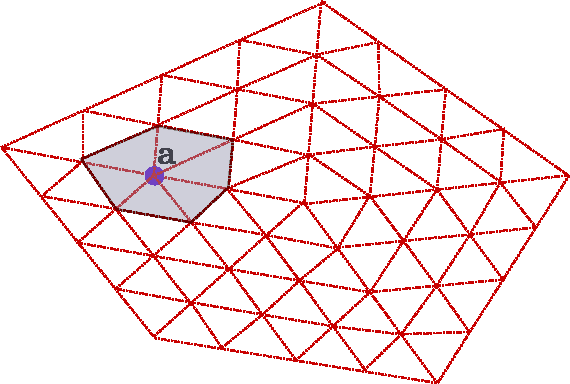
\includegraphics[width=0.84\textwidth]{patch_alg_5.pdf}
   % \end{overprint}
\end{figure}
\end{minipage}

\onslide<3>

\vspace{0.2 cm}
\textcolor{cadmiumgreen}{\textbf{Strategy for constructing the estimators}}
\begin{equation*}
%\label{eq:def:lambda:pos:neg}
\lambh^{\kk,\ii} \egaldef \lambh^{\kk,\ii,\mathrm{pos}} + \lambh^{\kk,\ii,\mathrm{neg}}, \quad \Ktildeghp \egaldef \left\{(\vunh,\vdeuxh) \in \Xghp \times \Xzerohp, \ \textcolor{electricpurple}{\vunh-\vdeuxh} \geq 0  \right\} \subset \Kg.
\end{equation*}
\textcolor{midnightblue}{\textbf{Nonconformity estimator 1:}}
\begin{equation*}
\eta_{\mathrm{nonc},1,K}^{\kk,\ii}  \egaldef  \tnorm{{\bm s}_h^{\kk,\ii}-\uh^{\kk,\ii}}_K, 
\end{equation*}
\vspace{-0.1 cm}
\textcolor{midnightblue}{\textbf{Nonconformity estimator 2:}}
\begin{equation*}
\eta_{\mathrm{nonc},2,K}^{\kk,\ii} \egaldef h_{\Omega} \CPF \left(\frac{1}{\mu_1} +
\frac{1}{\mu_2} \right)^{\frac{1}{2}} \left\| \lambh^{\kk,\ii,\mathrm{neg}}\right\|_K, 
\end{equation*}
\vspace{-0.2 cm}
\textcolor{midnightblue}{\textbf{Nonconformity estimator 3:}}
\begin{equation*}
\eta_{\mathrm{nonc},3,K}^{\kk,\ii}  \egaldef 2 h_{\Omega} \CPF \left(\frac{1}{\mu_1} +
\frac{1}{\mu_2} \right)^{\frac{1}{2}} \left\|\lambh^{\kk,\ii,\mathrm{pos}}\right\|_{\Omega}
\tnorm{{\bm s}_{h}^{\kk,\ii}-\uh^{\kk,\ii}}_K.
\end{equation*}

%%%%%%%

\onslide<4>
\textcolor{cadmiumgreen}{\textbf{Distinguishing the error components}}
\\
\textcolor{midnightblue}{\textbf{$p=1$}}
\vspace*{-0.6 cm}
\small{
\begin{equation*}
  \begin{split}
  \eta_{\mathrm{disc}}^{\kk,\ii} & := \left\{\sum_{\alpha=1}^2 \sum_{K \in \Th} \left(\eta_{\mathrm{disc},K,\alpha}^{\kk,\ii} + \eta_{\mathrm{osc},K,\alpha} \right)^2  \right\}^{\frac{1}{2}} + \left\{|\sum_{K \in \Th} \eta_{\mathrm{C},K}^{\kk,\ii,\mathrm{pos}} |  \right\}^{\frac{1}{2}} \\
  \eta_{\mathrm{lin}}^{\kk,\ii} & := \eta_{\mathrm{nonc}, 1}^{\kk,\ii} + \eta_{\mathrm{nonc}, 2}^{\kk,\ii} + \left(\eta_{\mathrm{nonc}, 3}^{\kk,\ii} \right)^{\frac{1}{2}}, \quad   \eta_{\mathrm{alg}}^{\kk,\ii} := \left\{\sum_{\alpha=1}^2 \sum_{K \in \Th} \left\| \mu_{\alpha}^{-\frac{1}{2}} {\bm \sigma}_{\alpha h, \mathrm{alg}}^{\kk,\ii} \right\|_K^2 \right\}^{\frac{1}{2}}
  \end{split}
\end{equation*}
\vspace*{-0.4 cm}
\textcolor{midnightblue}{\textbf{$p \geq 2$}}
\vspace*{-0.3 cm}
\begin{equation*}
  \begin{split}
    \eta_{\mathrm{disc}}^{\kk,\ii} & := \left\{\sum_{\alpha=1}^2 \sum_{K \in \Th} \left(\eta_{\mathrm{disc},K,\alpha}^{\kk,\ii} + \eta_{\mathrm{osc},K,\alpha} \right)^2  \right\}^{\frac{1}{2}}
    + \left\{2 |\left(\lambda_h^{\kk,\ii,\mathrm{pos}} - \lambda_h^{\kk,\ii}, u_{1h}^{\kk,\ii} - u_{2h}^{\kk,\ii} \right)_{\Omega} |  \right\}^{\frac{1}{2}} \\
    & + \tnorm{\tilde{\bs}_h^{\kk,\ii} - {\bs}_h^{\kk,\ii}}
    + C_{\Omega,\mu} \left\| \lambda_h^{\kk,\ii,\mathrm{neg}} - \tilde{\lambda}_{h}^{\kk,\ii,\mathrm{neg}} \right\|_{\Omega} + \left(2 C_{\Omega,\mu} \left\|\lambda_h^{\kk,\ii,\mathrm{pos}} \right\|  \right)^{\frac{1}{2}} \tnorm{\tilde{\bs}_h^{\kk,\ii} - {\bs}_h^{\kk,\ii}}^{\frac{1}{2}}\\
    \eta_{\mathrm{lin}}^{\kk,\ii} & := \tnorm{{\bs}_h^{\kk,\ii} - {\bu}_h^{\kk,\ii}} + C_{\Omega,\mu} \left\| \tilde{\lambda}_{h}^{\kk,\ii,\mathrm{neg}} \right\|_{\Omega} + \left(2 C_{\Omega,\mu} \left\|\lambda_h^{\kk,\ii,\mathrm{pos}} \right\|  \right)^{\frac{1}{2}}  \tnorm{{\bs}_h^{\kk,\ii} - {\bu}_h^{\kk,\ii}}^{\frac{1}{2}}
    \\
    & + \left\{2 |\left(\lambda_h^{\kk,\ii}, u_{1h}^{\kk,\ii} - u_{2h}^{\kk,\ii} \right)_{\Omega} | \right\}^{\frac{1}{2}}
  \end{split}
\end{equation*}
}
\onslide<5>

\vspace{0.1 cm}
\textcolor{cadmiumgreen}{\textbf{Parabolic weak formulation}}
\\\\
\textcolor{midnightblue}{\textbf{Weak formulation:}} 
For $\left(f_1,f_2\right) \in  [L^2(0,T;L^2(\Omega))]^2$, $\bu^0 \in H_g^1(\Omega) \times H_0^1(\Omega)$, 
find  $(u_1,u_2,\lambda) \in L^2(0,T;H_g^1(\Omega)) \times L^2(0,T;H_0^1(\Omega)) \times L^2(0,T; \Lambda)$ s.t. $\dps \partial_t \uialf \in L^2(0,T;H^{-1}(\Omega))$, and satisfying $\forall t \in \left]0,T\right[$ 
\begin{equation*}
\vspace{-0.2 cm}
\begin{split}
&\sum_{\ialf=1}^2 \langle \partial_t \uialf(t), \vialf \rangle + \sum_{\ialf=1}^2 \mu_\ialf \left(\nab \uialf(t), \nab \vialf \right)_{\Omega} - \left(\lambda(t),v_1-v_2\right)_{\Omega} = \sum_{\ialf=1}^2 \left(f_\ialf, \vialf \right)_{\Omega}, \hspace{0.15 cm} \forall \bv \in \left[H_0^1(\Omega)\right]^2 \\
& \left(\chi-\textcolor{carmine}{\lambda(t)}, \textcolor{electricpurple}{u_1(t)-u_2(t)}\right)_{\Omega} \geq 0 \quad \forall \chi \in \Lambda.
\end{split}
\end{equation*}
\textcolor{midnightblue}{\textbf{Discrete formulation:}}
Given $\left(u_{1h}^0,u_{2h}^0 \right) \in \Kgh^{p}$, search $(\uunhn,\udeuxhn,\lambh^n)\in \Xghp \times \Xzerohp \times
\Lahp$ such that for all $\left(z_{1h},z_{2h},\chi_h\right) \in \Xzerohp \times \Xzerohp \times \Lahp$ 
\begin{equation*}
\begin{array}{lcl}
\dps \frac{1}{\Dt_n} \sum_{\ialf=1}^2 \left(\uialfhn-\uialfh^{n-1}, z_{\ialf h}\right)_{\Omega} + \sum_{\ialf=1}^2 \mu_\ialf \left(\nab u_{\ialf h}^n, \nab z_{\ialf h}\right)_{\Omega}
- \left\langle \lambh^n, z_{1h}-z_{2h} \right \rangle_h
=  \dps \sum_{\ialf=1}^2 \left(f_\ialf,z_{\ialf h}\right)_{\Omega}, \\
\left\langle \chi_h - \textcolor{carmine}{\lambh^n}, \textcolor{electricpurple}{\uunh^n - \udeuxh^n}\right \rangle_h   \geq 0 
\end{array}
\end{equation*}

\onslide<6>
\vspace{0.2 cm}
\textcolor{red}{$\bm \gammalin= \bm \gammaalg \bm = {\bm {10^{-6}}}$}
\\\\
\textcolor{cadmiumgreen}{\hspace{2 cm} $t = 1.05 \times 10^5$ years \hspace{5 cm} $t = 3.5 \times 10^5$ years}
\begin{figure}
\centering
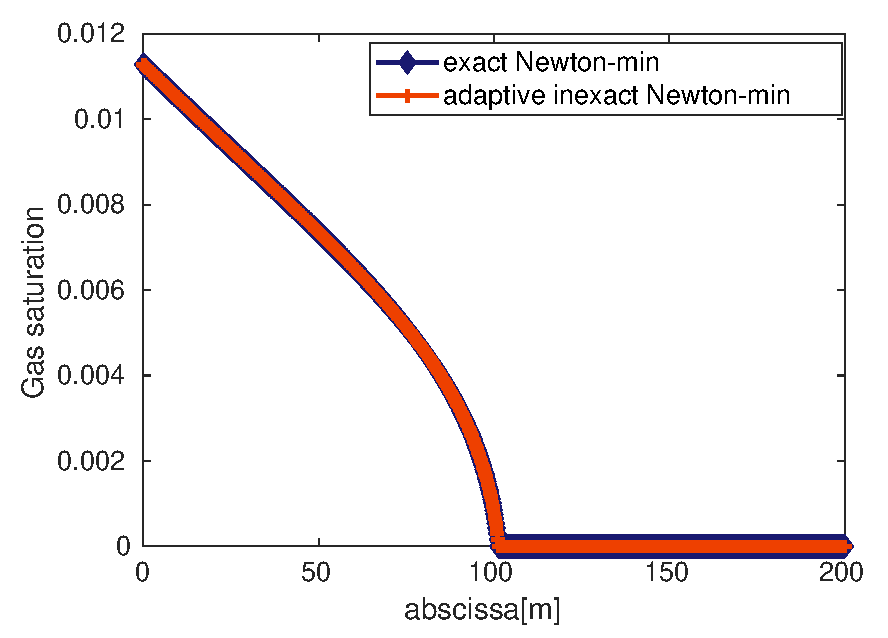
\includegraphics[width=0.48 \textwidth]{fig_article_chap_3/comparaison_plot_gas_saturations_exact_adapt_inexact_gamma_lin_10-6_gamma_alg_10-3_nt_21}
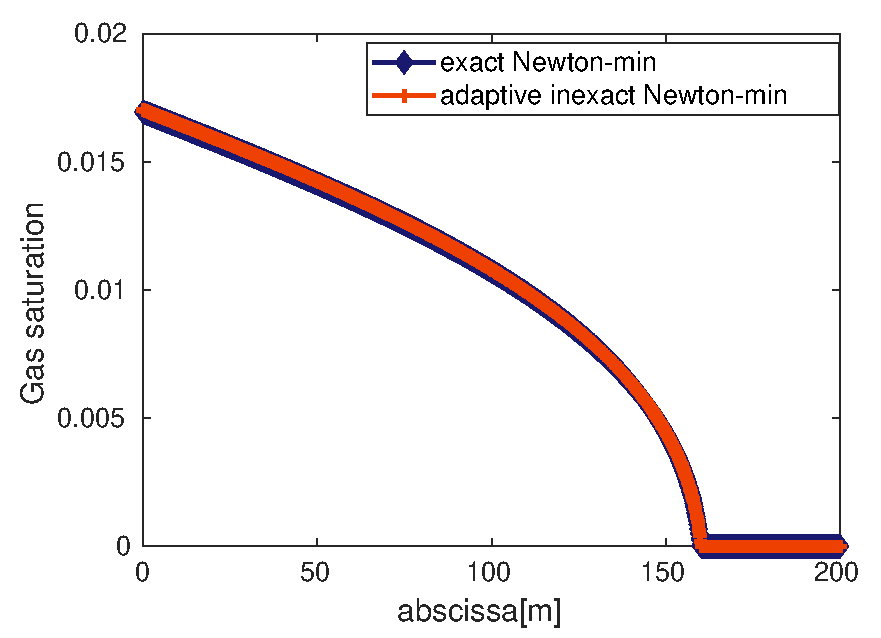
\includegraphics[width=0.48 \textwidth]{fig_article_chap_3/comparaison_plot_gas_saturations_exact_adapt_inexact_gamma_lin_gamma_alg_10-3_nt_70}
\end{figure}

 \end{overprint} 

\end{frame}
